
% \rlink expands to bare math; \rl is the text-mode-safe form used below.
\newcommand{\rl}[1]{\ensuremath{\rlink{#1}}}

\subsection{Two Worked Runs of The Tableau}\label{ss:ex}


Consider the formula $\mathrm{AG}\,\mu\wedge\mathrm{AG}(q\rightarrow\sigma)$ with $\mu=\tAU{\top}{q}{[1,4]}$, that is $\mathrm{AF}_{[1,4]}q$, and 
$\sigma=\tAR{\bot}{\neg q}{(0,3]}$, that is $\mathrm{AG}_{(0,3]}(\lnot q)$. The first conjunct demands a $q$ within
$[1,4]$ of every configuration; the second forbids a $q$ for $3$ time units after each one. The left conjunct proceeds as a persistent demand. Its first demand launches $\mu^\bullet$ with $x$
reset and the deadline $x\le\sup\kI=4$; the next re-demand meets a live pursuit, so \ruleref{Carry}
folds it in and the pursuit becomes $\mu^{\ast}$. Meanwhile the right conjunct re-imposes its body
$\neg q\vee\sigma$ at every configuration, so $N_2$ carries both, and the disjunction is settled
before $\mu^{\ast}$ is unfolded.
\noindent
Take $\neg q$, at $N_3$. The pursuit can then neither take \ruleref{Ustopcarry} nor \ruleref{Ugocarry}: \ruleref{Ustopcarry} would assert
$q$ into a goal set already holding $\neg q$, and \ruleref{Ugocarry} can only defer, which past $x=4$
empties the zone against the deadline. Both children close.
\noindent
Take $\sigma$ instead. It is launched with its own clock $z$ reset, and \ruleref{Ustopcarry} asserts
$q$, re-zeroing $x$ and recapping it at $b-a=3$; this is $N_4$, where the two clocks begin to run
together, $x=z$. That is the contradiction. The carried deadline $x\le3$ says the next $q$ is due
within $3$, while $\sigma$ forbids $q$ for as long as $z\in(0,3]$. At $N_5$ the \ruleref{Ustopcarry} branch needs a
$q$ it cannot have, and \ruleref{Ugocarry} needs $x>3$, which the deadline denies. Both children close,
so $N_2$ closes and the formula is \UNSAT.


\begin{figure}[h]
\centering
\begin{subfigure}[b]{0.5\textwidth}\centering
\resizebox{0.8\linewidth}{!}{%
\begin{tikzpicture}[
  every node/.style={align=center, font=\scriptsize},
  level 1/.style={sibling distance=26mm, level distance=9mm},
  level 2/.style={sibling distance=30mm, level distance=11mm},
  level 3/.style={sibling distance=15mm, level distance=11mm},
  level 4/.style={sibling distance=15mm, level distance=11mm},
  edge from parent/.style={draw,-}
]
\node {$N_0:\{\mathrm{AG}\,\mu\wedge\mathrm{AG}(q\!\rightarrow\!\sigma)\}\ \ANDn$}
 child { node {$N_1:\{\,\}$\\ $\OPEN$}
   edge from parent node[left,font=\tiny,pos=.45]{\rl{discharge}} }
 child { node {$N_2:\{\mu^{\ast},\neg q\vee\sigma\},\ x{:=}0$\\ $\Deadline{=}\{x\le 4\}\ \ORn$}
   child { node {$N_3:\{\neg q,\mu^{\ast}\}\ \ORn$}
     child { node {$\CLOSED$\\ $q\wedge\neg q$}
       edge from parent node[left,font=\tiny,pos=.45]{\rl{Ustopcarry}} }
     child { node {$\CLOSED$\\ $\rl{Ugocarry}$\\ needs $x>4$}
       edge from parent node[right,font=\tiny,pos=.45]{\rl{Ugocarry}} }
     edge from parent node[left,font=\tiny,pos=.45]{$\neg q$} }
  child { node {$N_4:\{q,\mu^{\ast},\sigma^\bullet\}$\\ $x{:=}0,\ z{:=}0,\ \Deadline{=}\{x\le3\}$}
     child { node {$N_5:\{\neg q,\mu^{\ast},\sigma^\bullet\}$\\ $x{=}z\in(0,3]\ \ORn$}
       child { node {$\CLOSED$\\ \rl{Ustopcarry} \\needs $q$}
         edge from parent node[left,font=\tiny,pos=.45]{\rl{Ustopcarry}} }
       child { node {$\CLOSED$\\ \rl{Ugocarry} \\needs $x>3$}
         edge from parent node[right,font=\tiny,pos=.45]{\rl{Ugocarry}} }
       edge from parent node[right,font=\tiny,pos=.45]{\rl{Delay}, \rl{EX}} }
     edge from parent node[right,font=\tiny,pos=.4]{$\sigma$; \rl{launch}, \rl{Ustopcarry}} }
   edge from parent node[right,font=\tiny,pos=.45]{$(\wedge)$, \rl{launch}, \rl{Carry}} };
\end{tikzpicture}}
\subcaption{$\mathrm{AG}(\mathrm{AF}_{[1,4]} q)\wedge\mathrm{AG}(q \rightarrow
\mathrm{AG}_{(0,3]}(\lnot q))$.}
\label{fig:ex-roll}
\end{subfigure}
\hfill
\begin{subfigure}[b]{0.48\textwidth}\centering
\resizebox{0.9\linewidth}{!}{%
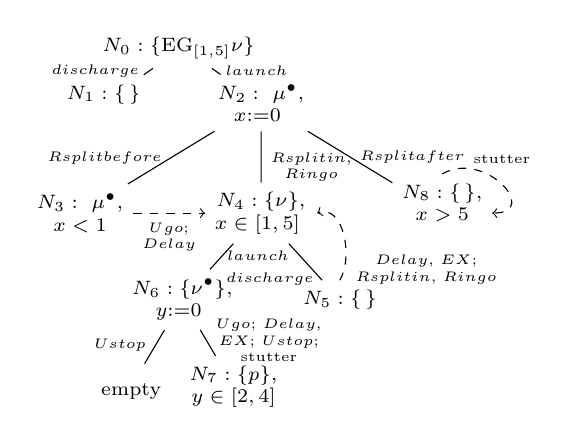
\begin{tikzpicture}[
  every node/.style={align=center, font=\scriptsize},
  level 1/.style={sibling distance=20mm, level distance=7mm},
  level 2/.style={sibling distance=23mm, level distance=14mm},
  level 3/.style={sibling distance=20mm, level distance=11mm},
  level 4/.style={sibling distance=13mm,level distance=11mm},
  edge from parent/.style={draw,-}
]
\node {$N_0:\{\mathrm{EG}_{[1,5]}\nu\}\ \ANDn$}
 child { node {$N_1:\{\,\}$\\ $\OPEN$}
   edge from parent node[left,font=\tiny,pos=.45]{\rl{discharge}} }
 child { node {$N_2:\ \mu^\bullet,$\\$x{:=}0\ \ANDn$}
   child { node (bef) {$N_3:\ \mu^\bullet,$\\$ x<1$}
    edge from parent node[left,font=\tiny,pos=.5]{\rl{Rsplitbefore}} }
   child { node (in) {$N_4:\{\nu\},$\\$ x\in[1,5]\ \ANDn$}
     child { node {$N_6:\{\nu^\bullet\},$\\$ y{:=}0\ \ORn$}
       child { node {$\CLOSED$\\ empty}
         edge from parent node[left,font=\tiny,pos=.45]{\rl{Ustop}} }
       child { node {$N_7:\{p\},$\\$ y\in[2,4]$}
         edge from parent node[right,font=\tiny,pos=.4]{\rl{Ugo}; \rl{Delay},\\ \rl{EX}; \rl{Ustop}; \\stutter} }
       edge from parent node[right,,xshift=-2pt,font=\tiny,pos=.45]{\rl{launch}} }
       child { node (disch) {$N_5:\{\,\}$}
       edge from parent node[left, yshift=-7pt,xshift=7pt,font=\tiny,pos=.45]{\rl{discharge}} }
     edge from parent node[right,font=\tiny,pos=.7]{\rl{Rsplitin},\\ \rl{Ringo}} }
   child { node (aft) {$N_8:\{\,\},$\\$ x>5$\\ $\OPEN$}
     edge from parent node[right,font=\tiny,pos=.5]{\rl{Rsplitafter}} }
   edge from parent node[right,font=\tiny,pos=.45]{\rl{launch}} };
\draw[->,dashed] (bef.east) to[out=0,in=180,looseness=.7]
  node[below,font=\tiny,pos=.5]{\rl{Ugo}; \\\rl{Delay}} (in.west);
\draw[->,dashed] (disch.north) to[out=60,in=20,looseness=1]
  node[right,yshift=-4pt,font=\tiny,pos=.25]{\rl{Delay}, \rl{EX};\\ \rl{Rsplitin}, \rl{Ringo} } (in.east);



\draw[->,dashed] (aft.north) to[out=30,in=0,looseness=2]
  node[above, yshift=4pt,font=\tiny]{stutter} (aft.east);
\end{tikzpicture}}
\subcaption{$\mathrm{EG}_{[1,5]}\tEU{\top}{p}{[2,4]}$.}\label{fig:ex-zeno}
\end{subfigure}
\caption{Two tableau runs. %$\ANDn$ marks an AND-node;$\ORn$ an OR-node. 
$\OPEN$ marks an open node, $\CLOSED$ a closed
one.}\label{fig:ex2}
\end{figure}

%\begin{example}%[A Zeno cycle that may be left]\label{ex:zeno}
Consider $\mathrm{EG}_{[1,5]}\,\nu$, where $\nu=\tEU{\top}{p}{[2,4]}$. Write $x$ for the clock of
the release, and $y$ for that of $\nu$. \ruleref{Cov} splits $N_0$ into a discharge child, which
carries no pursuit, and the launch $N_2$, where $x$ is reset. \ruleref{Rsplit} then partitions the zone,
conjunctively, into its three parts. At $N_3$, the \ruleref{Rsplitbefore} part, \ruleref{Delay} carries $x$ into  \kI. $N_8$, where $x>5$, drops $\mu^\bullet$ and leaves a goal-free node that
may delay indefinitely: a time-progressing loop, since no until needs to be fulfilled and $x$ is
extrapolated above $M$.
\noindent
$N_4$ represents the \ruleref{Rsplitin} part of \ruleref{Rsplit}, where $\nu$ is inserted into $\Gamma$ and so
demanded. \ruleref{Cov} applies, giving two conjunctive branches. The \ruleref{launch} child $N_6$
proves $\nu$. It carries $\nu^\bullet$ with $y$ reset; its \ruleref{Ustop} is empty there, the window
$[2,4]$ not yet open, so only \ruleref{Ugo} survives until a delay carries $y$ into $[2,4]$, where
\ruleref{Ustop} asserts $p$ and drops $\nu^\bullet$. The \ruleref{discharge} child $N_5$ drops $\nu$
from $\Gamma$ and carries $\mu^\bullet$ on; a delay and \ruleref{EX} revive the release, still inside
$[1,5]$, and its in-part demands $\nu$ once more. The search is back at $N_4$, closing a loop. That
loop is not time-progressing: $x$ is never reset, and the in-window zone holds it below $5$.
\noindent
Nonetheless, we can construct a successful marking  as $\mathcal M=\{N_0,\allowbreak N_1,\allowbreak N_2,\allowbreak N_3,\allowbreak N_4,\allowbreak N_5,\allowbreak N_6,\allowbreak N_7,\allowbreak N_8\}$. \ref{M2} holds because the only until pursuit is $\nu^\bullet$, active at $N_6$, and the path to
$N_7$ takes its \ruleref{Ustop} at a node whose zone meets $y\in[2,4]$. \ref{M1} holds because every node of
$\mathcal M$ reaches a time-progressing loop: the nodes carrying the release reach $N_8$ by delaying
until $x$ passes $5$, which lapses it, while $N_1$ and, once $\nu^\bullet$ is dropped, $N_7$ carry
no pursuit, so no deadline caps their delays and their stutter loops are time-progressing. So $\mathcal M$, as well as the tableau, are successful and
$\mathrm{EG}_{[1,5]}\,\nu$ is \SAT.
